\section{Date: 2026-11-04}
\noindent \textbf{Series ID: WPU054121013} 

\noindent This series is titled Producer Price Index by Commodity: Fuels and Related Products and Power: Residential Electric Power for East North Central Census Division and has a frequency of Monthly. The units are Index Dec 2007=100 and the seasonal adjustment is Not Seasonally Adjusted.The observation start date is 2007-12-01 and the observation end date is 2026-09-01.The popularity of this series is 1. \\ 

\noindent \textbf{Series ID: MRTSSM722USN} 

\noindent This series is titled Retail Sales: Food Services and Drinking Places and has a frequency of Monthly. The units are Millions of Dollars and the seasonal adjustment is Not Seasonally Adjusted.The observation start date is 1992-01-01 and the observation end date is 2026-08-01.The popularity of this series is 19. \\ 

\subsection{Raw Regression}
\noindent Regresses the two series against each other directly. A significant result here can come just as easily from both series sharing a long-run trend as from any real relationship.

\begin{center}
\begin{tabular}{lclc}
\toprule
\textbf{Dep. Variable:}            & value\_fred\_MRTSSM722USN & \textbf{  R-squared:         } &     0.737   \\
\textbf{Model:}                    &            OLS            & \textbf{  Adj. R-squared:    } &     0.734   \\
\textbf{Method:}                   &       Least Squares       & \textbf{  F-statistic:       } &     318.7   \\
\textbf{Date:}                     &      Wed, 04 Nov 2026     & \textbf{  Prob (F-statistic):} &  8.31e-35   \\
\textbf{Time:}                     &          22:07:01         & \textbf{  Log-Likelihood:    } &   -1192.6   \\
\textbf{No. Observations:}         &              116          & \textbf{  AIC:               } &     2389.   \\
\textbf{Df Residuals:}             &              114          & \textbf{  BIC:               } &     2395.   \\
\textbf{Df Model:}                 &                1          & \textbf{                     } &             \\
\textbf{Covariance Type:}          &         nonrobust         & \textbf{                     } &             \\
\bottomrule
\end{tabular}
\begin{tabular}{lcccccc}
                                   & \textbf{coef} & \textbf{std err} & \textbf{t} & \textbf{P$> |$t$|$} & \textbf{[0.025} & \textbf{0.975]}  \\
\midrule
\textbf{const}                     &   -2.164e+04  &     5164.973     &    -4.190  &         0.000        &    -3.19e+04    &    -1.14e+04     \\
\textbf{value\_fred\_WPU054121013} &     575.5062  &       32.238     &    17.852  &         0.000        &      511.643    &      639.370     \\
\bottomrule
\end{tabular}
\begin{tabular}{lclc}
\textbf{Omnibus:}       &  8.963 & \textbf{  Durbin-Watson:     } &    0.814  \\
\textbf{Prob(Omnibus):} &  0.011 & \textbf{  Jarque-Bera (JB):  } &   10.211  \\
\textbf{Skew:}          & -0.481 & \textbf{  Prob(JB):          } &  0.00606  \\
\textbf{Kurtosis:}      &  4.089 & \textbf{  Cond. No.          } & 1.25e+03  \\
\bottomrule
\end{tabular}
%\caption{OLS Regression Results}
\end{center}

Notes: \newline
 [1] Standard Errors assume that the covariance matrix of the errors is correctly specified. \newline
 [2] The condition number is large, 1.25e+03. This might indicate that there are \newline
 strong multicollinearity or other numerical problems.

\begin{figure}
\centering
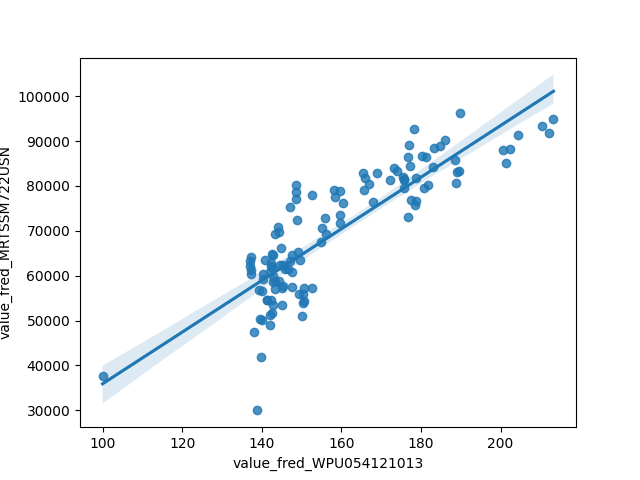
\includegraphics[scale = 0.9]{plots/plot_2026-11-04.png}
\caption{Raw Regression Plot for 2026-11-04}
\end{figure}
\newpage
\subsection{Detrended Regression}
\noindent Regresses the residuals of each series after removing its own linear time trend, so a shared trend can no longer drive the result on its own. A relationship that stays significant here is better evidence of a genuine link between the two series.

\begin{center}
\begin{tabular}{lclc}
\toprule
\textbf{Dep. Variable:}                       & value\_fred\_MRTSSM722USN\_detrended & \textbf{  R-squared:         } &     0.211   \\
\textbf{Model:}                               &                 OLS                  & \textbf{  Adj. R-squared:    } &     0.204   \\
\textbf{Method:}                              &            Least Squares             & \textbf{  F-statistic:       } &     30.56   \\
\textbf{Date:}                                &           Wed, 04 Nov 2026           & \textbf{  Prob (F-statistic):} &  2.08e-07   \\
\textbf{Time:}                                &               22:07:01               & \textbf{  Log-Likelihood:    } &   -1180.4   \\
\textbf{No. Observations:}                    &                   116                & \textbf{  AIC:               } &     2365.   \\
\textbf{Df Residuals:}                        &                   114                & \textbf{  BIC:               } &     2370.   \\
\textbf{Df Model:}                            &                     1                & \textbf{                     } &             \\
\textbf{Covariance Type:}                     &              nonrobust               & \textbf{                     } &             \\
\bottomrule
\end{tabular}
\begin{tabular}{lcccccc}
                                              & \textbf{coef} & \textbf{std err} & \textbf{t} & \textbf{P$> |$t$|$} & \textbf{[0.025} & \textbf{0.975]}  \\
\midrule
\textbf{const}                                &    1.527e-09  &      595.106     &  2.57e-12  &         1.000        &    -1178.899    &     1178.899     \\
\textbf{value\_fred\_WPU054121013\_detrended} &     318.6043  &       57.635     &     5.528  &         0.000        &      204.429    &      432.779     \\
\bottomrule
\end{tabular}
\begin{tabular}{lclc}
\textbf{Omnibus:}       & 41.308 & \textbf{  Durbin-Watson:     } &    0.835  \\
\textbf{Prob(Omnibus):} &  0.000 & \textbf{  Jarque-Bera (JB):  } &  110.393  \\
\textbf{Skew:}          & -1.327 & \textbf{  Prob(JB):          } & 1.07e-24  \\
\textbf{Kurtosis:}      &  6.975 & \textbf{  Cond. No.          } &     10.3  \\
\bottomrule
\end{tabular}
%\caption{OLS Regression Results}
\end{center}

Notes: \newline
 [1] Standard Errors assume that the covariance matrix of the errors is correctly specified.

\begin{figure}
\centering
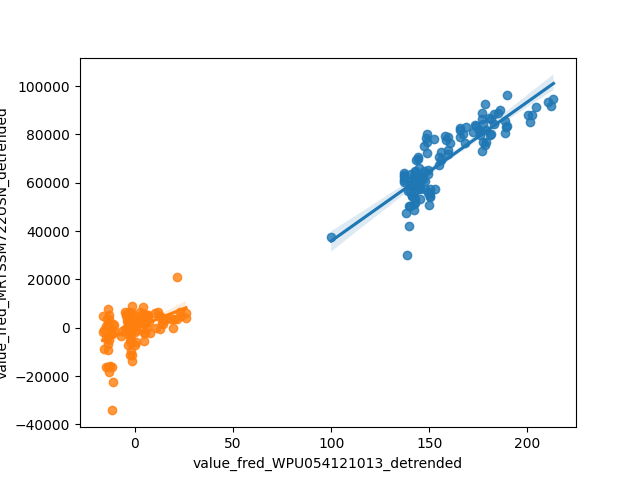
\includegraphics[scale = 0.9]{plots/plot_2026-11-04_detrended.png}
\caption{Detrended Regression Plot for 2026-11-04}
\end{figure}
\newpage
